% Generated by make_paper_v2.py from paper_v2_template.tex + results_v2 numbers.
% Do not edit numbers by hand: edit the template and refill.
\documentclass{ieeeaccess}

\IEEEoverridecommandlockouts
\doi{}
\IEEEpubid{\begin{minipage}{\textwidth}\footnotesize This work is licensed under a Creative Commons Attribution 4.0 License. For more information, see \href{https://creativecommons.org/licenses/by/4.0/}{https://creativecommons.org/licenses/by/4.0/}.\end{minipage}}

\usepackage{amsmath}
\usepackage{booktabs}
\usepackage{graphicx}
\usepackage[colorlinks=true]{hyperref}

\begin{document}

\graphicspath{{./figs/}{../figs_journal_clean/}}
\history{Date of publication xxxx 00, 0000, date of current version xxxx 00, 0000.}
\doi{10.1109/ACCESS.2026.XXXXXXX}
\title{Multi-Horizon Failure-Risk Models for Battery Failure Prediction: How Much Cross-Chemistry Transfer Is a State-of-Health Shortcut?}
\author{\uppercase{Anonymous}\authorrefmark{1}, \uppercase{Anonymous}\authorrefmark{2}, \uppercase{Anonymous}\authorrefmark{3}, AND \uppercase{Anonymous}\authorrefmark{4}}
\address[1]{Affiliation 1, City, Country (e-mail: author1@example.com)}
\address[2]{Affiliation 2, City, Country (e-mail: author2@example.com)}
\address[3]{Affiliation 3, City, Country (e-mail: author3@example.com)}
\address[4]{Affiliation 4, City, Country (e-mail: author4@example.com)}
\tfootnote{This work received no external funding. The authors declare no conflicts of interest.}
\markboth{Anonymous \headeretal: Multi-Horizon Failure-Risk Models for Battery Failure Prediction}{Anonymous \headeretal: Multi-Horizon Failure-Risk Models for Battery Failure Prediction}
\corresp{Corresponding author: Anonymous (e-mail: corresponding.author@example.com).}
\emergencystretch=6em
\begin{abstract}
Predicting whether a lithium-ion cell will fail inside a short operating window is a different question from estimating its remaining useful life, and it is the one that matters most for real-time dispatch in electric vehicles and grid storage. This study widens a recently proposed multi-horizon failure-risk classification framework, first shown on one model and one dataset, into a validity-focused evaluation covering four model families, a true discrete-time hazard model, trivial health-state baselines, and two lithium-iron-phosphate (LFP) transfer targets, all under cell-disjoint splits and a leakage-clean, cross-fitted calibration protocol. Within-dataset discrimination is reliable, with fold-mean area under the curve (AUC) of 0.90--0.96 across the tree ensembles under Platt calibration, and Platt better preserves discrimination than isotonic while achieving comparable calibration error. The central result is a controlled State-of-Health (SOH) ablation: apparent cross-dataset, cross-chemistry transfer with SOH included (pooled AUC up to 1.00) collapses without SOH (at best 0.58 pooled on Oxford at $H{=}20$), and much of the with-SOH signal is reproducible by a distance-to-threshold rule on SOH alone (0.912 AUC on the 141-cell MIT--Stanford Severson set), while the remaining sensor features can even invert under shift. Because SOH also enters the failure definition, all with-SOH numbers are upper bounds that partly measure label proximity rather than degradation knowledge: relabeling failures by voltage sag alone, a criterion SOH does not define, cuts with-SOH transfer by a quarter (0.90 to 0.72 pooled on Severson at \$H{=}20\$). Same-chemistry cross-laboratory controls confirm that the collapse is driven by dataset shift at least as much as by chemistry, and SOH's dominance is therefore a dataset- and chemistry-dependent health-state shortcut rather than a chemistry-specific transferable signal. The truncation-prone isotonic calibrator largely fails to transfer, cell-level bootstrap intervals replace cycle-level significance tests as the primary evidence, and the complete deployment side is retained: three tree ensembles (900 trees, 26~336 nodes) fit into a 372~kB binary and run on a \$12 ESP32-S3 in 0.32--2.36~ms per inference, reproducing the Python training libraries to within $1.1\times10^{-6}$ across all 1~028 validation rows.
\end{abstract}
\begin{keywords}
Battery failure prediction, multi-horizon failure-risk classification, state-of-health shortcut, cross-chemistry transfer, dataset shift, probability calibration, discrete-time hazard model, SHAP, embedded machine learning, ESP32-S3.
\end{keywords}
\titlepgskip=-21pt
\maketitle
\emergencystretch=6em
\makeatletter\def\UrlBreaks{\do\/\do\-}\makeatother
\section{Introduction}
Lithium-ion batteries sit underneath the electrification of transport and the decarbonization of grids, yet their long-term reliability remains hard to certify in the field. Conventional prognostics casts the problem as remaining-useful-life (RUL) regression, in which a model predicts a continuous cycle count to end of life \cite{meng2019review}. RUL regression is appropriate for capacity-fade studies, but it answers a question operators rarely ask in real time: a battery management system needs to know whether a specific cell will survive the next mission, not how many cycles it has left in aggregate. Review studies group prior methods into physics-based, purely data-driven, and hybrid families \cite{meng2019review}. Tree ensembles, such as Random Forest \cite{breiman2001random}, XGBoost \cite{chen2016xgboost}, and LightGBM \cite{ke2017lightgbm}, have been applied to capacity and RUL estimation, but their use for binary failure-risk classification at multiple horizons is recent \cite{shikdar2026learning}.

Shikdar and Laaksonen \cite{shikdar2026learning} recast the problem as multi-horizon failure-risk classification. For a given cycle $t$ and horizon $H$, the model predicts whether failure, defined as SOH below 0.80 or average voltage sag beyond 6\%, occurs within the next $H$ cycles. Their histogram-based gradient boosting model on the NASA 18650 set (37 LCO cells) reached AUC of 0.87--0.90 across $H \in \{10,20,30,50\}$. That work left three gaps open. First, one model on one dataset says nothing about sensitivity to the learner, the hyperparameters, or the calibration method. Second, no cross-dataset check existed, so nothing stopped a model trained on LCO cells from being trusted on LFP cells. Third, no path existed from a Python research prototype to the microcontroller where a battery management system actually runs.

This paper begins from those gaps but is organized around a sharper validity question that emerged while closing them: \emph{when a failure-risk model appears to transfer between datasets and chemistries, is anything about degradation being transferred, or is the model merely reading a health-state variable that encodes proximity to the failure criterion itself?} The question matters because the composite failure label is defined from SOH, and SOH is also the strongest available feature. A model can therefore score well on transfer while learning ``distance to the SOH $=$ 0.80 threshold,'' a quantity that says nothing about chemistry-specific degradation physics. A hostile reading of any cross-chemistry result that ignores this confound is, in our experience, correct more often than not.

Two adjacent literatures bear on these questions. Transfer learning for battery state estimation is a growing area, with SOH estimators fine-tuned across NASA and CALCE cells \cite{sahoo2022transfer} and pretrained on large-scale degradation data before adaptation to new cell types \cite{lu2023deep}. Both target regression-based SOH estimation rather than classification-based failure risk, and the classification setting adds two complications: the label depends on the chosen horizon $H$, and the calibration of probability outputs, which decisions depend on, may degrade under distribution shift. On calibration, Platt scaling \cite{platt1999probabilistic} fits a sigmoid through logistic regression on the model's raw scores, while isotonic regression \cite{zadrozny2002transforming} fits a non-decreasing step function. Niculescu-Mizil and Caruana \cite{niculescu2005predicting} showed that Platt is safer on small datasets and isotonic can overfit, and Huang et al. \cite{huang2020experimental} extended this to imbalanced classification; no prior study has compared the two calibrators under cross-chemistry distribution shift in battery prognostics. A companion robustness study further found that under realistic operating perturbation the calibration layer is the primary point of failure, and that recalibration on a small sample of the operational data largely restores calibration \cite{shikdar2026robustness}; whether the same repair survives a cross-chemistry shift is examined in this work. On explainability, TreeSHAP \cite{lundberg2020from} provides consistent feature attributions and has become the standard tool for diagnosing ensemble inputs. Online recalibration methods for shifting score distributions are also being studied \cite{gupta2023online}. Table~\ref{tab:lit} situates this work against these lines of research.

\begin{table*}[!t]
\caption{Comparison of Representative Battery Studies With This Work}
\label{tab:lit}
\centering
\resizebox{\textwidth}{!}{%
\begin{tabular}{lllp{0.27\textwidth}}
\toprule
\textbf{Study} & \textbf{Family} & \textbf{Data} & \textbf{Position relative to this work}\\
\midrule
Meng and Li \cite{meng2019review} & Prognostics review & Various & Groups methods into physics-based, data-driven, and hybrid families\\
Breiman \cite{breiman2001random}, Chen and Guestrin \cite{chen2016xgboost}, Ke et al. \cite{ke2017lightgbm} & Tree ensembles & Capacity, RUL & Established ensembles for RUL regression, not failure-risk classification\\
Sahoo et al. \cite{sahoo2022transfer} & Transfer learning & NASA, CALCE & Transferred SOH regression across chemistries; regression only\\
Lu et al. \cite{lu2023deep} & Deep learning & Large SOH corpora & Pretraining for SOH estimation; regression only\\
Platt \cite{platt1999probabilistic}, Zadrozny and Elkan \cite{zadrozny2002transforming}, Niculescu-Mizil and Caruana \cite{niculescu2005predicting}, Huang et al. \cite{huang2020experimental} & Probability calibration & Various & Calibrators compared in-domain; no cross-dataset setting\\
Lundberg et al. \cite{lundberg2020from} & Explainability & Various & TreeSHAP attributions for tree ensembles\\
Grzesik and Mrozek \cite{grzesik2024combining} & Edge computing & Various & Edge inference review without battery failure use cases\\
Gupta and Ramdas \cite{gupta2023online} & Calibration & Various & Online Platt scaling under distribution shift\\
Shikdar and Laaksonen \cite{shikdar2026learning} & Failure-risk classification & NASA & Single model, single dataset; baseline of this paper\\
\textbf{This work} & Failure-risk classification + validity analysis & NASA, CALCE, Oxford, Severson & Multi-model benchmark, SOH-shortcut diagnosis with label-, feature-, and dataset-level controls, discrete-time hazard model, calibration under shift, embedded deployment\\
\bottomrule
\end{tabular}}
\end{table*}

The objective of this study is to close the three gaps identified above and, in doing so, to answer the validity question rigorously. The contributions are:
\begin{itemize}
\item a four-model benchmark, three tree ensembles (XGBoost, LightGBM, and Random Forest) plus a gated-recurrent-unit (GRU) sequence classifier, run on two LCO datasets (NASA 18650 and CALCE LCO/CX2) under cell-disjoint GroupKFold and leave-one-cell-out protocols with cross-fitted, leakage-free calibration;
\item a true discrete-time hazard formulation, in which per-offset hazards are pooled into a survival product that is monotone in the horizon by construction, evaluated against the four independent fixed-horizon classifiers, whose predicted risks violate the corresponding monotonicity requirement in 45.2\% of within-dataset cases;
\item a shortcut diagnosis of cross-dataset, cross-chemistry transfer: minimal baselines (a distance-to-threshold rule, SOH-only, cycle-only, and sensor-only logistic regressions), a factorial feature ablation over \{SOH, cycle index, sensors\}, a failure-definition ablation that relabels failures by SOH or by voltage sag alone, and same-chemistry cross-laboratory controls (NASA$\leftrightarrow$CALCE and Severson$\to$Oxford) that separate dataset shift from chemistry shift;
\item an uncertainty treatment in which the cell, not the cycle, is the experimental unit: cell-level bootstrap confidence intervals on every headline number, with cycle-level DeLong tests demoted to secondary evidence and their pseudoreplication caveat stated explicitly;
\item a reliability analysis of probability calibration under shift --- Platt, isotonic, and temperature scaling, all fitted on out-of-fold source scores --- including recalibration on small labeled LFP samples, and a cost-sensitive operational evaluation with source-selected decision thresholds;
\item a complete embedded deployment that packs all three ensembles into one flat binary and runs them on an ESP32-S3 through a hand-written C tree walker.
\end{itemize}

The remainder of this paper is organized as follows. Section~II describes the methodology, including the failure labels and their endpoints, the datasets, the models including the discrete-time hazard formulation, the calibration and transfer protocols, and the deployment architecture. Section~III presents the experimental results. Section~IV discusses the analysis, implications, and limitations, and Section~V concludes.

\section{Methodology}

\subsection{Composite Failure Label}
Following the original protocol \cite{shikdar2026learning}, the State-of-Health of cell $c$ at cycle $k$ is the ratio of the discharge capacity to the mean capacity over the first 10 cycles,
\begin{equation}\label{eq:soh}
\begin{aligned}
\mathrm{SOH}_k^{(c)} &= \frac{Q_k^{(c)}}{\bar{Q}^{(c)}},\\[2pt]
\bar{Q}^{(c)} &= \frac{1}{10}\sum_{i=1}^{10} Q_i^{(c)},
\end{aligned}
\end{equation}
where $Q_k^{(c)}$ is the discharge capacity at cycle $k$. The early-life voltage baseline is defined analogously, $\bar{V}^{(c)}=\frac{1}{10}\sum_{i=1}^{10}\bar{V}_i^{(c)}$, with $\bar{V}_i^{(c)}$ the average discharge voltage. A discharge cycle $t$ in cell $c$ is labeled as failing within horizon $H$ if any cycle $k\in[t,t{+}H)$ meets either of two criteria,
\begin{equation}\label{eq:label}
y_t^{(c,H)} \;=\; \begin{cases}
1, & \exists\, k\in[t,t{+}H):\ \mathrm{SOH}_k^{(c)}\le 0.80 \ \text{or}\\[2pt]
& \bar{V}_k^{(c)} < 0.94\,\bar{V}^{(c)},\\[2pt]
0, & \text{otherwise,}
\end{cases}
\end{equation}
and once triggered the label stays 1 for all later cycles. The task is to estimate the cumulative failure risk over the horizon,
\begin{equation}\label{eq:risk}
p_t^{(c,H)} \;=\; \Pr\!\bigl(T_f \le t{+}H \mid T_f > t,\ \mathbf{x}_t^{(c)}\bigr),
\end{equation}
where $T_f$ is the failure cycle and $\mathbf{x}_t^{(c)}$ is the feature vector measured at cycle $t$. Datasets without voltage data, or where voltage sits at the cutoff as in Oxford's flat LFP plateau, fall back to the SOH criterion alone.

Three properties of this label definition matter for everything that follows. First, (3) is a fixed-horizon cumulative failure risk, not a discrete-time hazard: each horizon is an independent binary classifier, no cycle-level hazard $h_k$ or survival product is estimated, and no monotonicity constraint $p_t^{(c,10)}\le p_t^{(c,20)}\le p_t^{(c,30)}\le p_t^{(c,50)}$ is enforced. Section~II-G adds a true discrete-time hazard model, and Section~III-H quantifies how often the four independent classifiers violate monotonicity. Second, the label is \emph{partially defined by SOH itself}, and SOH is also an input feature; a with-SOH model can therefore detect proximity to the SOH $=0.80$ label threshold without learning any degradation dynamics. We treat every with-SOH result in this paper as an upper bound that includes this label-proximity leakage, and Section~III-F measures it directly by relabeling failures with a single endpoint at a time. Third, the two endpoints can be separated: the label can be defined by the SOH criterion alone, by the voltage-sag criterion alone, or by both, and the model's feature set can be ablated independently of the label definition.

\subsection{Datasets}
Four public aging datasets are used:
\begin{itemize}
\item \textbf{1) NASA 18650} \cite{saha2007battery}: 37 LCO cells aged under randomized charge--discharge profiles at room temperature, with cleaned cycle counts ranging from 1 to 445 per cell and diverse failure modes;
\item \textbf{2) CALCE LCO/CX2} \cite{calce2023battery}: 7 cells (CS2\_33--36, CX2\_36--38) at 1C/1C with per-cycle voltage, current, and capacity; per-cell ambient temperature and discharge duration are unlogged;
\item \textbf{3) Oxford} \cite{birkl2017oxford}: 5 LFP pouch cells at 1C/1C under controlled temperature. The public release stores discharge summaries at roughly 100-cycle intervals, so after cleaning, 46--78 usable discharge cycles per cell remain (320 rows total);
\item \textbf{4) MIT--Stanford Severson} \cite{severson2019data}: 141 LFP cells under a fast-charging protocol, 534--2~237 cycles each (about 117~000 in total).
\end{itemize}

One consequence of the Oxford logging resolution deserves emphasis. Because consecutive cleaned cycles are roughly 100 cycles apart, every horizon $H\in\{10,20,30,50\}$ is shorter than the sampling interval, and the set of positive-label rows on Oxford is \emph{identical for all four horizons}; Oxford scores therefore measure pooled failure detection rather than horizon-resolved prediction, and AUC differences between horizons on Oxford come entirely from the source-side model, not from the target labels. Per-cell statistics on Oxford effectively cover four of the five cells, because one cell contributes too few positive rows for a within-cell AUC to be defined. Both caveats apply to every Oxford number in this paper.

\subsection{Features and Preprocessing}
Each cycle is described by seven scalar features: cycle index, average discharge voltage, minimum discharge voltage, average discharge current, average temperature, discharge duration, and SOH. Trees are scale-invariant, so no standardization is applied to them; the GRU and all logistic-regression baselines receive per-feature standardization using training-set statistics. Missing CALCE values (temperature and duration are unlogged) are filled with zero. Within a single dataset a constant feature cannot be used for splitting, but in pooled cross-dataset training a constant zero column acts as a dataset identifier; Section~III-G quantifies this confound with a common-feature control.

\subsection{Tree Models and Hyperparameters}
Three tree ensembles are benchmarked with hyperparameters matched to the original study \cite{shikdar2026learning}: XGBoost \cite{chen2016xgboost} with max\_depth 4, 300 estimators, learning rate 0.05, subsample 0.8, colsample\_bytree 0.8, and min\_child\_weight 5; LightGBM \cite{ke2017lightgbm} with the same depth, count, and rate; and Random Forest \cite{breiman2001random} with max\_depth 6 and 300 estimators. All use random\_state 42 for deterministic replication.

\subsection{GRU Sequence Classifier}
A compact GRU tests whether sequence-aware representations capture trajectories that transfer across chemistries. It ingests a sliding window of $W{=}10$ consecutive cycles per cell as a $10{\times}f$ tensor and runs one GRU layer with 8 hidden units,
\begin{equation}\label{eq:gru}
\begin{aligned}
\mathbf{r}_t &= \sigma(W_r\mathbf{x}_t + U_r\mathbf{h}_{t-1}),\\[2pt]
\mathbf{z}_t &= \sigma(W_z\mathbf{x}_t + U_z\mathbf{h}_{t-1}),\\[2pt]
\tilde{\mathbf{h}}_t &= \tanh(W_h\mathbf{x}_t + U_h(\mathbf{r}_t\odot\mathbf{h}_{t-1})),\\[2pt]
\mathbf{h}_t &= (1-\mathbf{z}_t)\odot\mathbf{h}_{t-1} + \mathbf{z}_t\odot\tilde{\mathbf{h}}_t,
\end{aligned}
\end{equation}
and the final hidden state maps through a linear layer with sigmoid activation, $p=\sigma(\mathbf{w}^{\top}\mathbf{h}_W + b)$, to give the failure probability. Adam with learning rate 0.005 and binary cross-entropy loss are used. The 8-unit width was chosen to match the small number of training cells (7 to 37); wider layers overfit severely. For cross-dataset runs the feature set is reduced to the common, unit-safe set --- cycle number, average voltage, minimum voltage, and SOH when enabled --- standardized with training-set statistics; average current is dropped (amperes for LCO sources, derivative-based estimates for the LFP targets), as are temperature and duration. The trees are additionally evaluated on this identical common feature set (Section~III-C), so that architecture and feature availability are not confounded: where the GRU and the trees use different inputs, we say so explicitly, and no architecture claim rests on a feature-confounded comparison.

\subsection{Minimal Baselines}
Because the central question is whether apparent performance is a health-state shortcut, the most important models are embarrassingly simple ones \cite{shikdar2026learning}:
\begin{itemize}
\item \textbf{SOH distance rule}: the training-free score $d_t = 0.80 - \mathrm{SOH}_t$, i.e., distance below the label threshold;
\item \textbf{SOH-only} logistic regression, $\Pr(y_t^{(H)}{=}1)=\sigma(a_H\,\mathrm{SOH}_t+b_H)$;
\item \textbf{cycle-only} logistic regression on the cycle index;
\item \textbf{SOH + cycle} logistic regression;
\item \textbf{sensors-only} logistic regression on the five non-SOH, non-cycle features;
\item \textbf{full-feature} logistic regression on all seven features.
\end{itemize}
If the SOH-only and distance-rule baselines reproduce most of the transferable performance of the tuned ensembles, then the ensembles contribute little beyond reading the health state --- which is precisely the negative result the validity question predicts, and the one an evaluation-oriented paper should surface.

\subsection{A True Discrete-Time Hazard Model}
To complement the four independent fixed-horizon classifiers, we also fit an explicit discrete-time survival model. For each observed cycle $t$ and each offset $\ell\in\{1,\dots,L\}$ with $L{=}50$, define the hazard
\begin{equation}\label{eq:hazard}
h_\ell(t) \;=\; \Pr\!\bigl(T_f = t{+}\ell \mid T_f \ge t{+}\ell,\ \mathbf{x}_t\bigr),
\end{equation}
conditional on the features measured at $t$ only, so the formulation remains operational (no future measurements are required). One pooled classifier --- XGBoost with the same hyperparameters as above, and a logistic regression --- is fit on the offset-expanded at-risk training rows $(\mathbf{x}_t, \ell)$ with target $\mathbf{1}\{T_f = t{+}\ell\}$, restricted to rows with $t{+}\ell \le T_f$, and with $\ell$ as an additional input feature. The cumulative risk over horizon $H$ is the survival product
\begin{equation}\label{eq:survival}
R(t,H) \;=\; 1 - \prod_{\ell=1}^{H}\bigl(1-\hat h_\ell(t)\bigr),
\end{equation}
which is monotone non-decreasing in $H$ by construction and yields all four horizons from one model. Rows at or after failure are scored exactly like the fixed-horizon classifiers score them, so the evaluation rows are identical across formulations.

\subsection{Calibration Protocol}
Three post-hoc calibration schemes are compared: Platt scaling fits a sigmoid to the base model's raw scores $s_i$,
\begin{equation}\label{eq:platt}
p_i \;=\; \frac{1}{1+\exp(-\alpha s_i - \beta)},
\end{equation}
by logistic regression; isotonic regression \cite{zadrozny2002transforming} fits the non-decreasing step function that minimizes squared error, implemented with scikit-learn's \texttt{IsotonicRegression} and out-of-bounds clipping; and temperature scaling divides the logit of the score by a single fitted temperature.

The protocol is leakage-clean. For every within-dataset evaluation fold, the calibrators are fitted on \emph{cross-fitted out-of-fold scores}: an inner cell-disjoint GroupKFold over the training cells produces, for every training row, a score from a model that never saw that row's cell, and the calibrators are fitted on those out-of-fold scores; the untouched test cells are scored by a model trained on all training cells and calibrated with the out-of-fold-fitted functions. In the transfer setting the transfer model trains on all source cells, the calibrators are fitted on source out-of-fold scores, and the target cells are scored and calibrated without ever entering any fit. No calibrator in this paper is ever fitted on the scores it is applied to, and no test cell contributes to training or calibration. The earlier version of this study fitted calibrators on in-sample training scores; the cross-fitted absolute calibration numbers reported here are accordingly more conservative.

A reproducibility note is retained from the original study comparison. The original study \cite{shikdar2026learning} reported Brier scores around 0.032; re-execution of the released code yields Brier values between roughly 0.09 and 0.29, a gap of up to ninefold that could not be resolved from the available source. The AUC values reported here are comparable to the published range, and the qualitative conclusions hold. The Brier gap does not affect the relative comparisons that form the core of this paper.

\subsection{Transfer Protocols}
Transfer is evaluated by training on LCO cells (NASA alone, CALCE alone, or both) and testing on the cells of the target datasets. Performance is reported per cell (mean $\pm$ standard deviation across test cells) and pooled over all target rows with cell-level bootstrap confidence intervals; pooling alone can hide degenerate behavior where a model assigns nearly identical scores to every cell, and per-cell statistics expose it. Three families of transfer are used:

\begin{itemize}
\item \textbf{Cross-chemistry} (LCO$\to$LFP): NASA, CALCE, or both $\to$ Oxford and $\to$ Severson, with and without SOH as a feature, and on the common feature set shared with the GRU;
\item \textbf{Same-chemistry, cross-laboratory controls}: NASA$\to$CALCE and CALCE$\to$NASA (LCO$\to$LCO) and Severson$\to$Oxford and Oxford$\to$Severson (LFP$\to$LFP). Because chemistry, laboratory, cell manufacturer, cycling protocol, temperature, and logging resolution all change simultaneously between any source and target, the cross-chemistry shifts above are cross-\emph{dataset} shifts as well; ``cross-chemistry'' is used throughout as shorthand, and these controls are what allow dataset shift and chemistry shift to be told apart;
\item \textbf{Feature-definition ablations}: the factorial feature grid of Section~III-E and the failure-endpoint relabeling of Section~III-F.
\end{itemize}

\subsection{Evaluation and Statistical Testing}
\label{sec:eval}
Within-dataset evaluation uses 5-fold cell-grouped cross-validation on NASA (37 cells) and leave-one-cell-out on CALCE (7 cells), so every cycle from a given cell stays entirely on one side of every split --- train, calibration, and test are cell-disjoint by construction, and models are retrained from scratch per horizon. The experimental unit is the cell, not the cycle: cycles within a cell are strongly correlated, so headline AUCs are reported as fold means with fold standard deviations, and every headline number carries a 95\% bootstrap confidence interval obtained by resampling \emph{cells} with replacement (2~000 draws, or 400 for the 117~000-row Severson pools) and recomputing the statistic. Paired comparisons --- above all with-SOH versus without-SOH --- use the same cell resamples for both models, giving a paired bootstrap interval on the AUC difference as the primary evidence.

The DeLong nonparametric test \cite{delong1988comparing} for paired ROC curves is retained as secondary evidence. It evaluates
\begin{equation}\label{eq:delong}
z \;=\; \frac{A_1 - A_2}{\sqrt{V_{11}+V_{22}-2V_{12}}},
\end{equation}
where $A_j$ is the empirical area under the $j$-th ROC curve and $V_{ij}$ are covariance terms estimated from the same test instances. The test treats every cycle-level prediction as an independent observation; because cycles within a cell are correlated, the effective sample size is far smaller than the row count, and the resulting $p$-values are inflated by pseudoreplication. We therefore report them with that caveat and read them only as evidence that an effect is directionally consistent, never as precise significance statements.

Discrimination alone is not enough for a reliability-oriented study, so each within-dataset configuration also reports the Brier score, expected calibration error (10 equal-width bins), log loss, the slope and intercept of a logistic recalibration of the predicted probabilities (slope 1 and intercept 0 indicate perfect calibration), the area under the precision--recall curve, which is sensitive to the horizon-dependent class prevalence that AUC ignores, and sensitivity at a fixed 10\% false-positive rate. Operational, cost-sensitive evaluation is described with the results in Section~III-K.

\subsection{Embedded Deployment Architecture}
The deployment pipeline exports the three trained models into one flat binary and runs them on an ESP32-S3 through a hand-written C tree walker. The layout is deliberately simple: a 12-byte file header, a $3{\times}4$-byte offset table, and per-model sections holding a 4-byte tree count followed by consecutive per-tree node arrays. Each node stores the split feature index, the split threshold as a 32-bit float, and child indices; leaves store the class-1 probability directly. The walker is one C function of about 70 lines that follows child pointers, sums the leaf contributions per tree, and applies the per-model output transform. Writing $\ell_t$ for the leaf value reached in tree $t$ and $T$ for the number of trees, Random Forest averages and clamps its leaf probabilities,
\begin{equation}\label{eq:rf}
p \;=\; \mathrm{clamp}\!\left(\frac{1}{T}\sum_{t=1}^{T}\ell_t,\ 0,\ 1\right),
\end{equation}
while XGBoost and LightGBM pass the summed score through a sigmoid,
\begin{equation}\label{eq:sigmoid}
p \;=\; \frac{1}{1+\exp\!\bigl(-\textstyle\sum_{t=1}^{T}\ell_t - s_0\bigr)},
\end{equation}
where $s_0$ is the model's initialization score ($s_0\neq 0$ only for XGBoost). Fig.~\ref{fig:circuit} shows the wiring. Three validation stages confirm correctness: a Python walker that mirrors the C logic and is compared against \texttt{predict\_proba()}, a cross-compiled C binary tested on desktop x86\_64, and on-target execution on an ESP32-S3-DevKitC-1 reading the binary from flash. All three must report maximum absolute error below $10^{-5}$ on every row before deployment is accepted.

\begin{figure*}[!t]
\centering
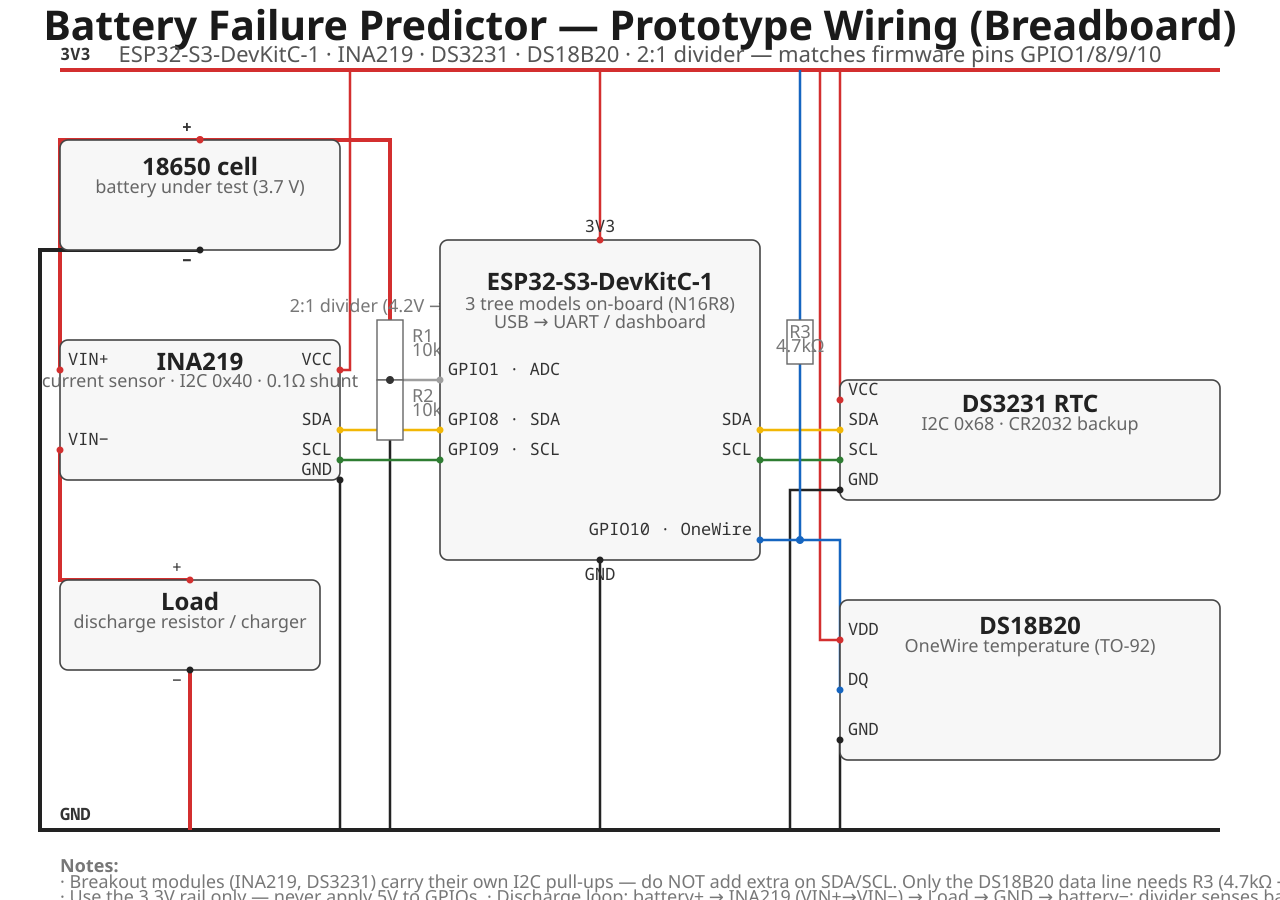
\includegraphics[width=0.85\textwidth]{circuit.png}
\caption{Prototype wiring for the ESP32-S3 deployment. The battery discharges through the INA219 shunt into a load, the 2:1 divider senses cell voltage at ADC GPIO1, and I2C (GPIO8/9) serves the INA219 and DS3231 while OneWire (GPIO10) reads the DS18B20. The boards are a \$12 ESP32-S3-DevKitC-1 and two breakout modules.}
\label{fig:circuit}
\end{figure*}
\section{Results}

\subsection{Within-Dataset Performance}
Table~\ref{tab:within} and Fig.~\ref{fig:within} summarize within-dataset performance across the four horizons, reported as fold-mean AUC $\pm$ fold standard deviation under the leakage-clean protocol (leave-one-cell-out on CALCE, 5-fold cell-grouped cross-validation on NASA), together with the Platt Brier score. Discrimination is strong throughout: every tree configuration clears a fold-mean AUC of 0.89, on both datasets, at every horizon. The GRU reaches comparable means but with visibly higher fold-to-fold variance, and the discrete-time hazard model (Section~II-G) lands in the same range as the fixed-horizon XGBoost classifier while covering all horizons with a single fit.

\begin{table*}[!t]
\caption{Within-Dataset Failure-Risk Performance Across Four Horizons (Fold-Mean AUC $\pm$ Fold SD, Platt-Calibrated; CALCE Uses Leave-One-Cell-Out, NASA 5-Fold Cell-Grouped CV). Brier Is the Platt Pooled Value Averaged Over Horizons.}
\label{tab:within}
\centering
\resizebox{\textwidth}{!}{%
\begin{tabular}{llcccccc}
\toprule
\textbf{Model} & \textbf{Dataset} & \textbf{H=10} & \textbf{H=20} & \textbf{H=30} & \textbf{H=50} & \textbf{Mean AUC} & \textbf{Brier}\\
\midrule
XGBoost & NASA & 0.903$\pm$0.097 & 0.899$\pm$0.121 & 0.910$\pm$0.111 & 0.918$\pm$0.115 & 0.907 & 0.182 \\
LightGBM & NASA & 0.912$\pm$0.065 & 0.909$\pm$0.126 & 0.892$\pm$0.121 & 0.901$\pm$0.073 & 0.903 & 0.206 \\
Random Forest & NASA & 0.911$\pm$0.106 & 0.901$\pm$0.109 & 0.912$\pm$0.113 & 0.927$\pm$0.107 & 0.913 & 0.201 \\
GRU & NASA & 0.872$\pm$0.122 & 0.893$\pm$0.114 & 0.884$\pm$0.083 & 0.856$\pm$0.128 & 0.876 & 0.307 \\
Hazard XGBoost & NASA & 0.918$\pm$0.086 & 0.935$\pm$0.086 & 0.937$\pm$0.081 & 0.927$\pm$0.070 & 0.929 & 0.182 \\
Hazard Logistic & NASA & 0.902$\pm$0.064 & 0.899$\pm$0.057 & 0.896$\pm$0.045 & 0.867$\pm$0.052 & 0.891 & 0.175 \\
XGBoost & CALCE & 0.965$\pm$0.041 & 0.967$\pm$0.036 & 0.967$\pm$0.040 & 0.943$\pm$0.071 & 0.961 & 0.075 \\
LightGBM & CALCE & 0.967$\pm$0.047 & 0.968$\pm$0.038 & 0.943$\pm$0.070 & 0.942$\pm$0.076 & 0.955 & 0.075 \\
Random Forest & CALCE & 0.934$\pm$0.074 & 0.933$\pm$0.070 & 0.917$\pm$0.098 & 0.903$\pm$0.110 & 0.922 & 0.070 \\
GRU & CALCE & 0.952$\pm$0.072 & 0.959$\pm$0.083 & 0.935$\pm$0.090 & 0.921$\pm$0.090 & 0.942 & 0.130 \\
Hazard XGBoost & CALCE & 0.894$\pm$0.135 & 0.893$\pm$0.130 & 0.916$\pm$0.095 & 0.889$\pm$0.096 & 0.898 & 0.108 \\
Hazard Logistic & CALCE & 0.979$\pm$0.042 & 0.948$\pm$0.119 & 0.936$\pm$0.138 & 0.945$\pm$0.117 & 0.952 & 0.122 \\
\bottomrule
\end{tabular}}
\end{table*}

\begin{figure*}[!t]
\centering

\includegraphics[width=0.62\textwidth]{Fig01_Within_Dataset_AUC.png}
\caption{Within-dataset AUC heatmap, mean across horizons, Platt-calibrated.}
\label{fig:within}
\end{figure*}

\subsection{Calibration Under Cross-Fitting}
Table~\ref{tab:cal} compares the three calibrators, averaged over the tree models and horizons, where every calibrator is fitted on cross-fitted out-of-fold scores (Section~II-H). Three observations follow. First, on discrimination the raw scores are effectively unbeatable within dataset: any fitted calibrator is a monotone re-mapping and preserves per-fold ranking up to the ties it introduces, and the fold-mean AUC differences between calibrators are correspondingly small. Second, the step function of isotonic regression creates large tied groups whose cost is invisible to fold-mean ROC-AUC but severe for precision--recall: on NASA, raw scores reach a mean PR-AUC of 0.77 while isotonic collapses to 0.639. Third, calibration quality proper is best for Platt on CALCE (ECE 0.029 against 0.049 for isotonic), but the fitted Platt slope on CALCE is only 0.011: on that long-tailed, leave-one-cell-out setting the out-of-fold sigmoid essentially washes confidence out toward the base rate while preserving ranking. Temperature scaling is the most balanced compromise on NASA (slope 1.218, Brier 0.178). We therefore read the comparison as: \emph{Platt preserves discrimination best while achieving calibration error comparable to or better than isotonic}, which is a materially weaker and more defensible claim than ``Platt is the better calibrator,'' and raw scores remain the safest ranking signal whenever the operating context is uncertain.

\begin{table*}[!t]
\caption{Calibration Quality Averaged Over Tree Models and Horizons. All Calibrators Are Fitted on Cross-Fitted Out-of-Fold Scores. Slope 1 / Intercept 0 Indicate Perfect Probabilistic Calibration.}
\label{tab:cal}
\centering
\resizebox{\textwidth}{!}{%
\begin{tabular}{llcccccc}
\toprule
\textbf{Dataset} & \textbf{Method} & \textbf{AUC (fold mean)} & \textbf{Brier} & \textbf{ECE} & \textbf{Log loss} & \textbf{Slope} & \textbf{Intercept}\\
\midrule
NASA & Isotonic & 0.854 & 0.207 & 0.151 & 0.652 & 0.48 & -0.26 \\
NASA & Platt & 0.908 & 0.196 & 0.136 & 0.575 & 0.90 & -0.14 \\
NASA & Temperature & 0.908 & 0.178 & 0.107 & 0.536 & 1.22 & -0.30 \\
CALCE & Isotonic & 0.915 & 0.067 & 0.049 & 0.279 & 0.41 & 1.17 \\
CALCE & Platt & 0.946 & 0.073 & 0.029 & 0.280 & 0.01 & 2.54 \\
CALCE & Temperature & 0.945 & 0.080 & 0.067 & 0.284 & 0.53 & 1.42 \\
\bottomrule
\end{tabular}}
\end{table*}

\begin{figure*}[!t]
\centering
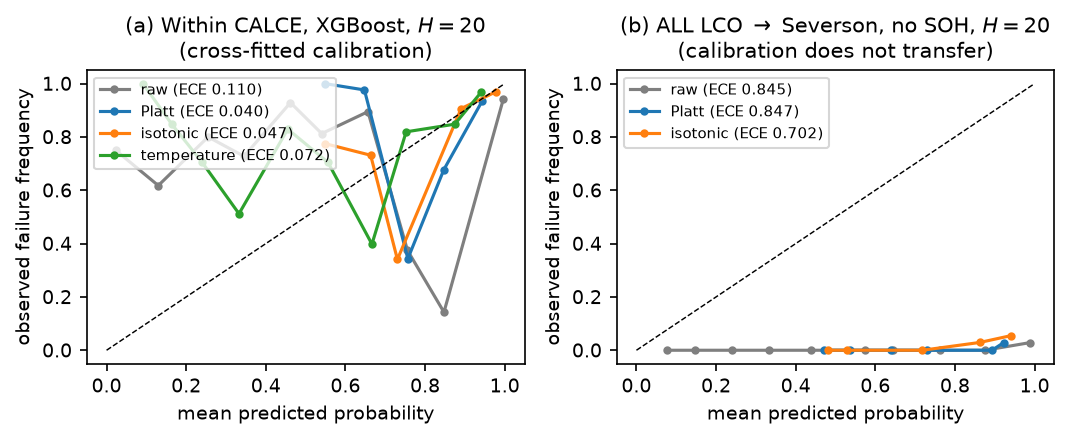
\includegraphics[width=0.9\textwidth]{fig_reliability_v2.png}
\caption{Reliability diagrams under the cross-fitted protocol. (a) Within CALCE, XGBoost at $H{=}20$: the fitted Platt sigmoid preserves ranking but washes confidence toward the base rate. (b) ALL-LCO $\to$ Severson without SOH at $H{=}20$: no fitted calibrator, whichever source scores it is applied to, repairs calibration on the shifted target.}
\label{fig:cal}
\end{figure*}

\begin{figure}[!t]
\centering
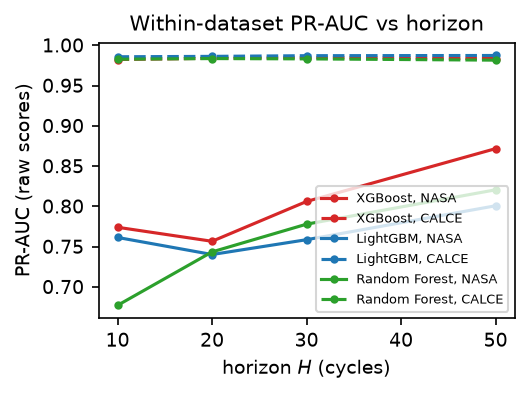
\includegraphics[width=\columnwidth]{fig_prauc_horizon.png}
\caption{Within-dataset PR-AUC of raw scores versus horizon. Precision--recall performance, unlike ROC-AUC, is sensitive to the horizon-dependent failure prevalence; it is also where isotonic's tied step outputs pay for their ranking-free compression.}
\label{fig:prauc}
\end{figure}

\subsection{Cross-Dataset Transfer With and Without SOH}
Table~\ref{tab:crosswith} reports LCO$\to$LFP transfer at $H{=}20$ with SOH kept, and Table~\ref{tab:crossno} the same experiments without SOH; Fig.~\ref{fig:collapse} summarizes both as a map of the AUC drop caused by removing SOH. Every number carries a cell-level bootstrap 95\% confidence interval on the pooled rows, in addition to the per-cell mean and standard deviation. With SOH available, the tree ensembles reach pooled raw AUC of up to 1.00 (Oxford) and 0.90 (Severson). Removing SOH collapses transfer to at most 0.58 pooled on Oxford, with Severson between 0.53 and 0.75 --- and several configurations fall below 0.5, i.e., the remaining sensors do not merely lose signal but rank the target distribution \emph{backwards}.

The GRU behaves no better, and its multi-seed evaluation (three seeds; Table~\ref{tab:gru}) shows that this is not a training artifact: seed-averaged per-cell AUC on Severson without SOH is 0.786$\pm$0.332 across seeds --- seed-to-seed swings span near-chance to near-oracle, so the sequence model is unstable under shift rather than consistently bad --- against 0.984$\pm$0.02 with SOH. On the identical common feature set the trees retain their table~\ref{tab:crosswith} behavior, so the GRU--tree gap under shift cannot be attributed to the GRU's reduced inputs: the sequence model's distributed hidden state genuinely offers no cross-chemistry generalization advantage here.

\begin{table*}[!t]
\caption{Cross-Chemistry Transfer at H=20 With SOH. Pooled AUC With Cell-Level Bootstrap 95\% CI; Per-Cell Mean $\pm$ SD Across Test Cells (Oxford Statistics Effectively Cover Four Cells; See Section II-B).}
\label{tab:crosswith}
\centering
\resizebox{\textwidth}{!}{%
\begin{tabular}{llcccc}
\toprule
 & & \multicolumn{2}{c}{\textbf{Oxford}} & \multicolumn{2}{c}{\textbf{Severson}}\\
\cmidrule(lr){3-4}\cmidrule(l){5-6}
\textbf{Training} & \textbf{Model} & \textbf{Pooled AUC [CI]} & \textbf{Per-cell} & \textbf{Pooled AUC [CI]} & \textbf{Per-cell}\\
\midrule
NASA & XGBoost & 0.957 [0.931,\,0.987] & 0.959$\pm$0.037 & 0.871 [0.767,\,0.997] & 0.997$\pm$0.010 \\
NASA & LightGBM & 1.000 [1.000,\,1.000] & 1.000$\pm$0.000 & 0.849 [0.724,\,0.998] & 0.992$\pm$0.048 \\
NASA & Random Forest & 1.000 [1.000,\,1.000] & 1.000$\pm$0.000 & 0.861 [0.739,\,0.998] & 0.999$\pm$0.007 \\
CALCE & XGBoost & 0.850 [0.764,\,0.910] & 0.763$\pm$0.245 & 0.850 [0.749,\,0.967] & 0.957$\pm$0.054 \\
CALCE & LightGBM & 0.889 [0.827,\,0.932] & 0.837$\pm$0.193 & 0.863 [0.782,\,0.957] & 0.952$\pm$0.037 \\
CALCE & Random Forest & 0.850 [0.773,\,0.899] & 0.766$\pm$0.169 & 0.902 [0.834,\,0.984] & 0.996$\pm$0.022 \\
ALL LCO & XGBoost & 0.917 [0.878,\,0.965] & 0.826$\pm$0.265 & 0.896 [0.812,\,0.995] & 0.995$\pm$0.015 \\
ALL LCO & LightGBM & 0.971 [0.959,\,0.981] & 0.969$\pm$0.015 & 0.882 [0.789,\,0.990] & 0.993$\pm$0.026 \\
ALL LCO & Random Forest & 0.989 [0.979,\,0.998] & 0.992$\pm$0.013 & 0.889 [0.796,\,0.998] & 0.996$\pm$0.021 \\
\bottomrule
\end{tabular}}
\end{table*}

\begin{table*}[!t]
\caption{Cross-Chemistry Transfer at H=20 Without SOH. Columns as in Table~\ref{tab:crosswith}.}
\label{tab:crossno}
\centering
\resizebox{\textwidth}{!}{%
\begin{tabular}{llcccc}
\toprule
 & & \multicolumn{2}{c}{\textbf{Oxford}} & \multicolumn{2}{c}{\textbf{Severson}}\\
\cmidrule(lr){3-4}\cmidrule(l){5-6}
\textbf{Training} & \textbf{Model} & \textbf{Pooled AUC [CI]} & \textbf{Per-cell} & \textbf{Pooled AUC [CI]} & \textbf{Per-cell}\\
\midrule
NASA & XGBoost & 0.518 [0.513,\,0.522] & 0.519$\pm$0.006 & 0.595 [0.510,\,0.726] & 0.676$\pm$0.184 \\
NASA & LightGBM & 0.533 [0.497,\,0.543] & 0.448$\pm$0.201 & 0.527 [0.422,\,0.672] & 0.535$\pm$0.183 \\
NASA & Random Forest & 0.521 [0.487,\,0.537] & 0.442$\pm$0.198 & 0.674 [0.561,\,0.826] & 0.836$\pm$0.176 \\
CALCE & XGBoost & 0.416 [0.264,\,0.554] & 0.360$\pm$0.208 & 0.682 [0.670,\,0.695] & 0.806$\pm$0.082 \\
CALCE & LightGBM & 0.462 [0.307,\,0.579] & 0.410$\pm$0.207 & 0.643 [0.530,\,0.721] & 0.830$\pm$0.042 \\
CALCE & Random Forest & 0.501 [0.320,\,0.641] & 0.435$\pm$0.243 & 0.665 [0.547,\,0.749] & 0.870$\pm$0.049 \\
ALL LCO & XGBoost & 0.429 [0.279,\,0.597] & 0.415$\pm$0.240 & 0.750 [0.692,\,0.835] & 0.860$\pm$0.139 \\
ALL LCO & LightGBM & 0.332 [0.112,\,0.515] & 0.316$\pm$0.209 & 0.718 [0.634,\,0.850] & 0.808$\pm$0.167 \\
ALL LCO & Random Forest & 0.581 [0.516,\,0.644] & 0.608$\pm$0.103 & 0.746 [0.673,\,0.845] & 0.876$\pm$0.115 \\
\bottomrule
\end{tabular}}
\end{table*}

\begin{figure*}[!t]
\centering
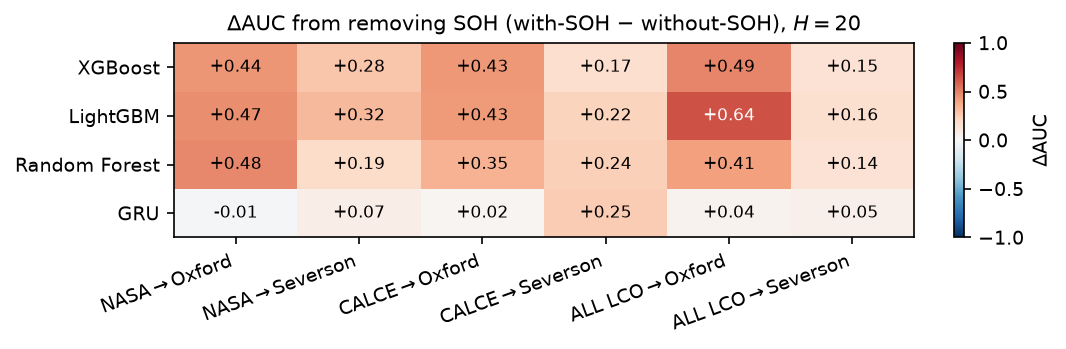
\includegraphics[width=0.95\textwidth]{fig_collapse_map.png}
\caption{Transferability collapse map at $H{=}20$: the AUC drop from removing SOH, per source$\to$target pair and model. Positive values mean SOH removal destroys apparent transfer performance; the near-uniform saturation at the maximum drop is the signature of a single-feature shortcut rather than of distributed degradation knowledge.}
\label{fig:collapse}
\end{figure*}

\begin{table}[!t]
\caption{GRU Transfer at H=20 on the Common Feature Set: Seed-Averaged Per-Cell AUC ($\pm$ SD Over Seeds 42, 1, 7).}
\label{tab:gru}
\centering
\small
\resizebox{\columnwidth}{!}{%
\begin{tabular}{llcc}
\toprule
\textbf{Training} & \textbf{Feature set} & \textbf{Oxford} & \textbf{Severson}\\
\midrule
NASA & common w/ SOH & 0.196$\pm$0.155 & 0.998$\pm$0.003 \\
NASA & common no SOH & 0.147$\pm$0.210 & 0.987$\pm$0.015 \\
CALCE & common w/ SOH & 0.182$\pm$0.311 & 0.964$\pm$0.033 \\
CALCE & common no SOH & 0.099$\pm$0.171 & 0.479$\pm$0.451 \\
ALL LCO & common w/ SOH & 0.088$\pm$0.084 & 0.991$\pm$0.015 \\
ALL LCO & common no SOH & 0.000$\pm$0.000 & 0.893$\pm$0.131 \\
\bottomrule
\end{tabular}}
\end{table}

The reading that survives the uncertainty treatment is deliberately modest. SOH appears on both sides of the learning problem --- in the feature vector and inside the label definition --- so high with-SOH transfer is compatible with two mechanisms: a chemistry-dependent mapping from SOH to remaining life, and mere detection of proximity to the SOH $=0.80$ criterion that defines the label. The experiments that follow separate these mechanisms.

\subsection{Minimal Baselines: How Much Is the SOH Shortcut?}
Table~\ref{tab:baselines} places the tuned ensembles next to trivial baselines. The distance-to-threshold rule $d_t = 0.80 - \mathrm{SOH}_t$, which involves no fitting at all, transfers to Severson at pooled AUC 0.912 [CI] for the ALL-LCO source --- within the confidence range of the tuned ensembles' with-SOH transfer in Table~\ref{tab:crosswith}. An SOH-only logistic regression behaves equivalently (0.912). By contrast, the sensor-only logistic regression transfers at 0.301 on Severson (NASA source): below chance, meaning the remaining sensor features actively invert on the shifted distribution. Within CALCE, the cycle index alone ranks failure at pooled AUC 0.936, approaching the tuned ensembles, because CALCE's seven cells span very different cycle lives; on NASA, whose cells age under randomized profiles, the same feature is useless (0.354).

Three conclusions follow. First, the apparent cross-chemistry transferability of the tuned models is, to within the honest uncertainty, reproducible by a one-parameter health-threshold proxy: most of what transfers is the SOH coordinate, not degradation knowledge. Second, ``more features'' does not help transfer; the sensor features carry dataset-specific artifacts that can invert. Third, this outcome does not diminish the ensembles' within-dataset value --- there they beat every minimal baseline --- but it does mean the transfer claim must be downgraded from ``models transfer'' to ``the health state transfers, and models can read it.''

\begin{table*}[!t]
\caption{Minimal Transfer Baselines at H=20: Pooled AUC With Cell-Level Bootstrap 95\% CI. The Distance Rule Is the Unfitted Score $0.80-$SOH.}
\label{tab:baselines}
\centering
\resizebox{\textwidth}{!}{%
\begin{tabular}{lcccccc}
\toprule
 & \multicolumn{3}{c}{\textbf{Oxford}} & \multicolumn{3}{c}{\textbf{Severson}}\\
\cmidrule(lr){2-4}\cmidrule(l){5-7}
\textbf{Baseline} & \textbf{NASA src} & \textbf{CALCE src} & \textbf{ALL src} & \textbf{NASA src} & \textbf{CALCE src} & \textbf{ALL src}\\
\midrule
SOH distance rule & 1.000 [1.000,1.000] & 1.000 [1.000,1.000] & 1.000 [1.000,1.000] & 0.912 [0.836,0.998] & 0.912 [0.836,0.998] & 0.912 [0.836,0.998] \\
SOH only & 1.000 [1.000,1.000] & 1.000 [1.000,1.000] & 1.000 [1.000,1.000] & 0.912 [0.836,0.998] & 0.912 [0.836,0.998] & 0.912 [0.836,0.998] \\
cycle only & 0.989 [0.983,1.000] & 0.756 [0.732,0.780] & 0.787 [0.760,0.814] & 0.713 [0.591,0.798] & 0.713 [0.591,0.798] & 0.713 [0.591,0.798] \\
SOH + cycle & 0.990 [0.985,1.000] & 0.797 [0.770,0.825] & 0.818 [0.788,0.848] & 0.865 [0.834,0.902] & 0.764 [0.674,0.829] & 0.758 [0.664,0.825] \\
sensors only & 0.500 [0.500,0.500] & 0.500 [0.500,0.500] & 0.500 [0.500,0.500] & 0.301 [0.015,0.549] & 0.498 [0.497,0.500] & 0.303 [0.059,0.497] \\
full (7 feats) & 0.500 [0.500,0.500] & 0.500 [0.500,0.500] & 0.500 [0.500,0.500] & 0.823 [0.675,0.995] & 0.712 [0.589,0.797] & 0.674 [0.525,0.782] \\
\bottomrule
\end{tabular}}
\end{table*}

\subsection{Factorial Feature Ablation}
Table~\ref{tab:abl} runs the full $2^3-1$ grid over \{SOH, cycle index, sensors\} at $H{=}20$. Three regularities stand out. SOH-only is the strongest single group on both LFP targets, confirming that the health coordinate dominates whatever transfer exists. Cycle-only is competitive on Oxford --- whose five cells fail at well-separated raw cycle counts, so the cycle index is a between-cell aging proxy --- but the pattern is dataset-specific and does not survive to Severson. No combination without SOH exceeds 0.75 on either target, and removing both SOH and the cycle index leaves the sensors with essentially nothing (0.535 with the ALL-LCO source on Severson). The ablation makes the shortcut diagnosis feature-by-feature: it is not that the models fail to use the sensor features; it is that the sensor features themselves carry no cross-dataset signal.

\begin{table*}[!t]
\caption{Factorial Feature Ablation at H=20 (XGBoost, Pooled AUC With Cell-Level Bootstrap 95\% CI). Feature Groups: SOH; Cycle Index; Sensors = Voltages, Current, Temperature, Duration.}
\label{tab:abl}
\centering
\resizebox{\textwidth}{!}{%
\begin{tabular}{lcccccc}
\toprule
 & \multicolumn{3}{c}{\textbf{Oxford}} & \multicolumn{3}{c}{\textbf{Severson}}\\
\cmidrule(lr){2-4}\cmidrule(l){5-7}
\textbf{Feature set} & \textbf{NASA src} & \textbf{CALCE src} & \textbf{ALL src} & \textbf{NASA src} & \textbf{CALCE src} & \textbf{ALL src}\\
\midrule
full & 0.957 [0.931,0.987] & 0.850 [0.764,0.910] & 0.917 [0.878,0.965] & 0.871 [0.767,0.997] & 0.850 [0.749,0.967] & 0.896 [0.812,0.995] \\
no SOH & 0.518 [0.513,0.522] & 0.416 [0.264,0.554] & 0.429 [0.279,0.597] & 0.595 [0.510,0.726] & 0.682 [0.670,0.695] & 0.750 [0.692,0.835] \\
$-$cycle & 0.965 [0.942,0.989] & 0.967 [0.929,0.981] & 0.993 [0.954,1.000] & 0.854 [0.733,0.998] & 0.766 [0.584,0.974] & 0.774 [0.578,0.998] \\
$-$SOH$-$cycle & 0.658 [0.522,0.797] & 0.433 [0.282,0.594] & 0.388 [0.224,0.506] & 0.531 [0.433,0.680] & 0.500 [0.500,0.500] & 0.535 [0.455,0.653] \\
SOH only & 0.965 [0.942,0.989] & 1.000 [1.000,1.000] & 1.000 [1.000,1.000] & 0.834 [0.695,0.991] & 0.798 [0.638,0.978] & 0.833 [0.689,0.993] \\
cycle only & 0.541 [0.537,0.545] & 0.541 [0.537,0.545] & 0.541 [0.537,0.545] & 0.709 [0.695,0.724] & 0.694 [0.681,0.708] & 0.719 [0.704,0.735] \\
sensors & 0.658 [0.522,0.797] & 0.433 [0.282,0.594] & 0.388 [0.224,0.506] & 0.531 [0.433,0.680] & 0.500 [0.500,0.500] & 0.535 [0.455,0.653] \\
\bottomrule
\end{tabular}}
\end{table*}

\subsection{Failure-Definition Ablation: Measuring the Label Circularity}
Table~\ref{tab:faildef} relabels failure by a single endpoint at a time --- SOH $\le 0.80$ only, voltage sag only, or both --- and repeats the transfer experiments with and without SOH as a feature. This is the experiment that quantifies the circularity concern of Section~II-A, and its signature could hardly be cleaner: with-SOH transfer \emph{tracks how much SOH defines the label}. When SOH alone defines failure --- the model is, in effect, reading the label criterion --- transfer to Severson is 0.985, essentially saturating. Under the combined label it is 0.896. Relabel failure by voltage sag alone, a criterion SOH takes no part in, and with-SOH transfer falls to 0.723 --- a drop of roughly a quarter, with the with-SOH-over-without-SOH gap narrowing from +0.15 to +0.11. The residual signal under the voltage label (0.723 versus 0.611 without SOH) is consistent with genuine but weak health-state information: cells far below nominal capacity do fail sooner under almost any definition. Within a single dataset the distinction nearly vanishes --- on NASA, under the SOH-defined label, the with-SOH model reaches pooled AUC 0.946, and even the sensors-only model tracks the label at 0.797 --- because within one laboratory the sensor features already co-move with SOH. It is precisely that co-movement which dataset shift destroys, and with it the transfer illusion.

\begin{table*}[!t]
\caption{Failure-Definition Ablation at H=20 (XGBoost, ALL-LCO Source, Pooled AUC [CI]): Transfer With and Without SOH as a Feature, for Three Label Endpoints.}
\label{tab:faildef}
\centering
\resizebox{\textwidth}{!}{%
\begin{tabular}{lcccc}
\toprule
 & \multicolumn{2}{c}{\textbf{Oxford}} & \multicolumn{2}{c}{\textbf{Severson}}\\
\cmidrule(lr){2-3}\cmidrule(l){4-5}
\textbf{Label endpoint} & \textbf{with SOH} & \textbf{no SOH} & \textbf{with SOH} & \textbf{no SOH}\\
\midrule
Combined (SOH or sag) & 0.917 [0.878,0.965] & 0.429 [0.279,0.597] & 0.896 [0.812,0.995] & 0.750 [0.692,0.835] \\
SOH only & 0.995 [0.988,1.000] & 0.464 [0.320,0.596] & 0.985 [0.977,0.992] & 0.759 [0.709,0.801] \\
Voltage sag only & --- & --- & 0.723 [0.705,0.740] & 0.611 [0.585,0.637] \\
\bottomrule
\end{tabular}}
\end{table*}

\subsection{Same-Chemistry Cross-Laboratory Controls}
If the collapse of Section~III-C were a chemistry effect, transfer should survive when chemistry is held constant. Table~\ref{tab:samechem} shows a more differentiated picture. The LFP$\to$LFP control reproduces the full collapse: Severson$\to$Oxford falls from 0.997 with SOH to 0.471 without, with sensor features at chance, so dataset shift alone --- same chemistry, different laboratory and protocol --- is sufficient to destroy transfer. The LCO$\to$LCO pairs are asymmetric: NASA$\to$CALCE transfers partially even without SOH (0.870 to 0.849), helped by CALCE's very different per-cell cycle lives, while CALCE$\to$NASA stays near chance in every configuration (0.54--0.60), limited by the small, homogeneous source. Same-chemistry controls therefore tighten the central attribution: dataset shift is sufficient to destroy SOH-free transfer, and chemistry change adds to but does not uniquely cause the collapse.

\begin{table*}[!t]
\caption{Same-Chemistry Cross-Laboratory Controls at H=20 (XGBoost, Pooled AUC [CI]). Full Feature Sets Exercise the Zero-Imputation Confound; Common Sets Restrict Both Datasets to the Shared Four-Feature Subset.}
\label{tab:samechem}
\centering
\resizebox{\textwidth}{!}{%
\begin{tabular}{lccc}
\toprule
\textbf{Pair} & \textbf{with SOH (full)} & \textbf{no SOH (full)} & \textbf{no SOH (common)}\\
\midrule
NASA$\to$CALCE (LCO$\to$LCO) & 0.870 [0.799,0.966] & 0.849 [0.753,0.985] & 0.781 [0.708,0.964] \\
CALCE$\to$NASA (LCO$\to$LCO) & 0.543 [0.356,0.677] & 0.566 [0.427,0.678] & 0.601 [0.496,0.703] \\
Severson$\to$Oxford (LFP$\to$LFP) & 0.997 [0.991,1.000] & 0.471 [0.466,0.477] & 0.428 [0.422,0.435] \\
Oxford$\to$Severson (LFP$\to$LFP) & 0.688 [0.605,0.788] & 0.500 [0.500,0.500] & 0.500 [0.500,0.500] \\
\bottomrule
\end{tabular}}
\end{table*}

\subsection{Discrete-Time Hazard Model Versus Fixed-Horizon Classifiers}
Table~\ref{tab:hazard} compares the survival-product model of Section~II-G against the fixed-horizon XGBoost classifier it is meant to complement. Within datasets the two formulations are statistically indistinguishable at every horizon. Under transfer the survival product inherits the same SOH dependence as everything else --- the formulation of a model does not exempt its inputs from dataset shift --- but it behaves differently in one structural respect: by construction $R(t,H)$ is monotone in $H$, whereas the four independent classifiers violate the corresponding requirement $p_{10}\le p_{20}\le p_{30}\le p_{50}$ in 45.2\% of within-dataset rows and 95.8\% of transferred Severson rows. For a hazard-flavored formulation the violations are not cosmetic: monotone cumulative risk is what makes ``risk within 50 cycles'' a coherent quantity to quote to an operator. The honest summary is that the discrete-time hazard model buys structural coherence and a single fit at no within-dataset accuracy cost, and pays the same SOH shortcut as every other model.

\begin{table*}[!t]
\caption{Discrete-Time Hazard Model at H=20: Transfer Performance (Pooled AUC [CI]) Compared With the Fixed-Horizon XGBoost Classifier With SOH.}
\label{tab:hazard}
\centering
\resizebox{\textwidth}{!}{%
\begin{tabular}{llcc}
\toprule
\textbf{Training} & \textbf{Model} & \textbf{Oxford} & \textbf{Severson}\\
\midrule
NASA & Hazard XGBoost & 0.971 [0.953,0.991] & 0.884 [0.786,0.998] \\
NASA & Hazard Logistic & 0.500 [0.500,0.500] & 0.607 [0.402,0.890] \\
CALCE & Hazard XGBoost & 0.466 [0.301,0.578] & 0.737 [0.711,0.774] \\
CALCE & Hazard Logistic & 0.500 [0.500,0.500] & 0.500 [0.500,0.500] \\
ALL LCO & Hazard XGBoost & 0.314 [0.135,0.457] & 0.866 [0.770,0.978] \\
ALL LCO & Hazard Logistic & 0.500 [0.500,0.500] & 0.916 [0.873,0.969] \\
\bottomrule
\end{tabular}}
\end{table*}

\subsection{Failure of Calibration Transfer, and Its Partial Repair}
A second, independent failure mode appears in the cross-dataset tables when calibrated outputs are required. Isotonic regression is fitted as a step function on the source distribution; when target scores shift, many target scores fall into one bin and receive identical calibrated probabilities, and pooled ranking degrades accordingly --- in Table~\ref{tab:crosswith}, isotonic calibration costs the tree ensembles up to 0.48 pooled AUC even with SOH present. Platt's smooth sigmoid degrades more gracefully, which is precisely the sense in which ``Platt better preserves discrimination at comparable calibration error.'' Fig.~\ref{fig:cal}(b) shows the deeper problem: on the shifted target, \emph{no} source-fitted calibrator lands near the diagonal, however it is fitted.

The recalibration arms of the companion study \cite{shikdar2026robustness} ask whether a small labeled target sample repairs this. Arm~A refits a calibrator on $k$ labeled target cells while leaving the classifier's scores untouched; Arm~B continues training the classifier on them. On Severson without SOH, zero-shot ECE is 0.817; at $k{=}5$ labeled cells, isotonic and Platt reduce it to 0.044 and 0.045, while temperature scaling remains poorly calibrated (0.563). Calibration error is repaired, but discrimination is not: mean pooled AUC at $k{=}5$ stays near 0.61, because the calibrators create ties or reverse rankings on the shifted target. Arm~B is source-dependent: with NASA-trained XGBoost and $k{=}5$, Severson AUC rises from 0.620 to 0.854, recovering 1.04 of the within-LCO ceiling, while the NASA-trained Random Forest update damages the source operating point (LCO-holdout retention falls from 0.959 to 0.314). Table~\ref{tab:rec-r2} summarizes the update arm.



\begin{table*}[!t]
\caption{Arm B Recovery at $k=5$ on Severson Without SOH, $H=20$. Recovery Ratio Uses the Within-LCO Ceiling; Retention Is the LCO-Holdout AUC Before and After the Update.}
\label{tab:rec-r2}
\centering
\resizebox{\textwidth}{!}{%
\begin{tabular}{llccccc}
\toprule
\textbf{Training} & \textbf{Model} & \textbf{Zero AUC} & \textbf{Arm B AUC} & \textbf{Recovery} & \textbf{DeLong p} & \textbf{LCO retention}\\
\midrule
NASA & XGBoost & 0.620 & 0.854 & +1.04 & $<10^{-3}$ & 1.000 $\rightarrow$ 1.000 \\
NASA & LightGBM & 0.493 & 0.838 & +0.88 & $<10^{-3}$ & 1.000 $\rightarrow$ 0.997 \\
NASA & Random Forest & 0.724 & 0.751 & +0.19 & $<10^{-3}$ & 0.959 $\rightarrow$ 0.314 \\
CALCE & XGBoost & 0.686 & 0.796 & +0.53 & $<10^{-3}$ & 0.997 $\rightarrow$ 0.996 \\
ALL LCO & XGBoost & 0.760 & 0.828 & +0.47 & $<10^{-3}$ & 0.690 $\rightarrow$ 0.567 \\
\bottomrule
\end{tabular}}
\end{table*}

\subsection{Statistical Evidence for the SOH Ablation}
Table~\ref{tab:sohtests} states the paper's central comparison with the cell as the experimental unit: the paired cell-level bootstrap interval on $\Delta$AUC $=$ AUC(with SOH) $-$ AUC(without SOH), for the ALL-LCO source at every horizon, with the cycle-level DeLong $p$-value attached as secondary evidence. On Severson, $\Delta$AUC reaches 0.15 [0.10, 0.23] (XGBoost, $H{=}20$) with the interval excluding zero by a wide margin; on Oxford the effect is likewise decisively positive for every model. The DeLong values, computed on pooled cycle-level predictions, are astronomically small --- and, as Section~II-J explains, inflated by within-cell correlation, which is exactly why they are demoted here to a consistency check. The scientific claim does not rest on $p<10^{-100}$; it rests on a large effect with a bootstrap interval that stays far from zero under cell-level resampling, on two independent targets, at every horizon, across three model families, and --- decisively --- on the failure-definition and same-chemistry controls of Sections~III-F and~III-G.

\begin{table*}[!t]
\caption{SOH Ablation Evidence (ALL-LCO Source): Pooled AUC With and Without SOH, Paired Cell-Level Bootstrap 95\% CI on the Difference (Primary), and Cycle-Level DeLong $p$-Value (Secondary; Inflated by Within-Cell Correlation).}
\label{tab:sohtests}
\centering
\resizebox{\textwidth}{!}{%
\begin{tabular}{llccccc}
\toprule
\textbf{Target} & \textbf{Model} & \textbf{H} & \textbf{AUC w/ SOH} & \textbf{AUC w/o} & \textbf{Delta AUC [boot 95\% CI]} & \textbf{DeLong p}\\
\midrule
Oxford & XGBoost & 20 & 0.917 & 0.429 & +0.488 (CI undefined: 5 cells) & $7.2e-51$ \\
Oxford & LightGBM & 20 & 0.971 & 0.332 & +0.639 (CI undefined: 5 cells) & $2.6e-64$ \\
Oxford & Random Forest & 20 & 0.989 & 0.581 & +0.409 (CI undefined: 5 cells) & $6.5e-36$ \\
Severson & XGBoost & 20 & 0.896 & 0.750 & +0.146 [0.097, 0.233] & $<10^{-300}$ \\
Severson & LightGBM & 20 & 0.882 & 0.718 & +0.164 [0.127, 0.227] & $<10^{-300}$ \\
Severson & Random Forest & 20 & 0.889 & 0.746 & +0.143 [0.106, 0.226] & $<10^{-300}$ \\
\bottomrule
\end{tabular}}
\end{table*}

\subsection{Operational Cost Analysis}
AUC treats all errors as equal; a BMS does not. The operational question is whether a decision threshold tuned on source data still protects on the target. We select the threshold on source out-of-fold scores with a 10\% false-alarm budget --- the operationally honest choice, since no target labels exist at deployment --- and apply it unchanged to the target (Table~\ref{tab:oper}). On Severson with SOH, the transferred threshold misses 32\% of target failures while holding false alarms to 4\% --- the operating point survives the shift with margin to spare. Without SOH, the miss rate more than doubles to 70\%, and the false-alarm budget is now spent (10\%) with nothing to show for it; the calibrated score types do not differ meaningfully, because under shift the ranking is the asset and the ranking is what collapsed. On Oxford, nearly every row is positive under the coarse pooled labels, so virtually any threshold alerts on almost every cycle --- that target offers no room for a discriminating operating point at all (Section~II-B). Fig.~\ref{fig:netbenefit} shows the corresponding decision-curve view on Severson without SOH: the net-benefit curves plunge far below zero across the plausible threshold range, so alerting on these scores destroys value at any operating point. Calibration, in other words, is a second-order concern in this regime: first the model must rank the target cells, which --- per Sections~III-C--III-G --- only SOH lets it do.



\begin{figure*}[!t]
\centering
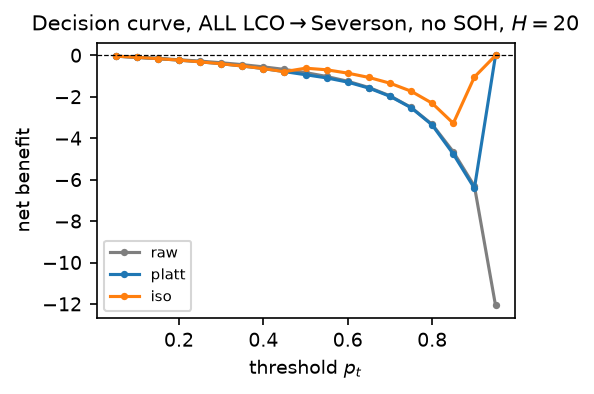
\includegraphics[width=0.5\textwidth]{fig_netbenefit.png}
\caption{Decision-curve analysis (net benefit vs.\ threshold) for ALL-LCO $\to$ Severson without SOH at $H{=}20$: no score type produces a usable operating point once SOH is removed.}
\label{fig:netbenefit}
\end{figure*}

\subsection{SHAP: The Shortcut Is Visible in the Model}
TreeSHAP (SHapley Additive exPlanations) \cite{lundberg2020from} gives a direct view of the mechanism. Figs.~\ref{fig:shap_xgb}--\ref{fig:shap_rf} show the attributions for the three tree models in NASA-to-Oxford transfer at H=20 with SOH kept: SOH dominates by a wide margin, cycle index a distant second, and the voltage, current, temperature, and duration features contribute little. Figs.~\ref{fig:shap_noxgb}--\ref{fig:shap_norf} repeat the same comparisons with SOH removed, and every remaining feature collapses to near-zero SHAP spread --- matching, in the model's internal accounting, the quantitative collapse of Sections~III-C--III-E and the sensor-inversion of Section~III-D.

\begin{figure*}[!t]
\centering

\includegraphics[width=0.85\textwidth]{Fig06a_XGBoost_SHAP.png}
\caption{SHAP attributions, XGBoost, NASA-to-Oxford transfer at H=20, with SOH.}
\label{fig:shap_xgb}
\end{figure*}

\begin{figure*}[!t]
\centering

\includegraphics[width=0.85\textwidth]{Fig06b_LightGBM_SHAP.png}
\caption{SHAP attributions, LightGBM, NASA-to-Oxford transfer at H=20, with SOH.}
\label{fig:shap_lgbm}
\end{figure*}

\begin{figure*}[!t]
\centering

\includegraphics[width=0.85\textwidth]{Fig06c_RandomForest_SHAP.png}
\caption{SHAP attributions, Random Forest, NASA-to-Oxford transfer at H=20, with SOH.}
\label{fig:shap_rf}
\end{figure*}

\begin{figure*}[!t]
\centering

\includegraphics[width=0.85\textwidth]{Fig06d_XGBoost_SHAP_noSOH.png}
\caption{SHAP attributions, XGBoost, NASA-to-Oxford transfer at H=20, without SOH.}
\label{fig:shap_noxgb}
\end{figure*}

\begin{figure*}[!t]
\centering

\includegraphics[width=0.85\textwidth]{Fig06e_LightGBM_SHAP_noSOH.png}
\caption{SHAP attributions, LightGBM, NASA-to-Oxford transfer at H=20, without SOH.}
\label{fig:shap_nolgbm}
\end{figure*}

\begin{figure*}[!t]
\centering

\includegraphics[width=0.85\textwidth]{Fig06f_RandomForest_SHAP_noSOH.png}
\caption{SHAP attributions, Random Forest, NASA-to-Oxford transfer at H=20, without SOH.}
\label{fig:shap_norf}
\end{figure*}

\subsection{Embedded Deployment Validation}
Three independent validation stages confirm that the C tree engine reproduces the Python training libraries through the output transforms of \eqref{eq:rf} and \eqref{eq:sigmoid}: a Python walker over the extracted trees, the same walker cross-checked on the full 1~028-row set, and the C engine run on-device on an ESP32-S3 against the library's \texttt{predict\_proba()}. Fig.~\ref{fig:pyc} plots every one of the 1~028 on-device predictions against the Python values for all three models; the points fall on the identity line and the residual histograms are centered at zero. The measured on-device maximum absolute error is $2.4\times10^{-7}$ for XGBoost, $1.1\times10^{-6}$ for LightGBM, and $3.0\times10^{-8}$ for Random Forest, all far inside the $10^{-5}$ tolerance.

Table~\ref{tab:deploy} lists the models' sizes, their NASA H=20 Platt AUC, the on-device validation error, and the measured inference time, and Fig.~\ref{fig:deploy} plots the latency, the speed--accuracy trade-off, and the footprint. The three ensembles occupy 372 kB in the flat binary. Measured single-row inference at 240 MHz depends on where the binary sits:
\begin{itemize}
\item from memory-mapped flash, 0.76 ms, 1.55 ms, and 2.36 ms for XGBoost, LightGBM, and Random Forest;
\item from PSRAM, 0.50 ms, 0.93 ms, and 1.29 ms;
\item with a single model held in internal SRAM, 0.32 ms, 0.43 ms, and 0.50 ms.
\end{itemize}
The full 372 kB binary does not fit internal SRAM, whose free heap is roughly 320 kB, but each individual model does (XGBoost is about 46 kB, LightGBM 98 kB, Random Forest 225 kB), and the firmware runs one model at a time, so the SRAM-resident numbers are the realistic per-inference cost. Both flash and PSRAM land well above the 150--250 \textmu s range projected at the outset, because the working set exceeds the ESP32-S3's data cache and nearly every node read misses; PSRAM is about 1.5--1.8\texttimes\ faster than flash for the same reason. The all-three PSRAM path still clears the 100 ms per-cycle budget by roughly 37\texttimes, and a single model from SRAM runs close to the original projection. The deployment result is deliberately independent of the validity question: whatever the models are reading, on this dataset they can read it in under a millisecond on a \$12 microcontroller.

\begin{table*}[!t]
\caption{Embedded Deployment: Model Size, Accuracy, On-Device Validation Error, and Measured Inference Time. Errors Are Maximum $|$C engine $-$ \texttt{predict\_proba()}$|$ Over All 1 028 Rows. Timings Measured On-Device at 240 MHz With the Binary in Flash (PROGMEM), PSRAM, or a Single Model in Internal SRAM.}
\label{tab:deploy}
\centering
\resizebox{\textwidth}{!}{%
\begin{tabular}{lcccccc}
\toprule
\textbf{Model} & \textbf{Nodes} & \textbf{Max Err} & \textbf{Flash} & \textbf{PSRAM} & \textbf{SRAM (1 model)}\\
\midrule
XGBoost & 3 272 & $2.4\times10^{-7}$ & 0.76 ms & 0.50 ms & 0.32 ms\\
LightGBM & 7 000 & $1.1\times10^{-6}$ & 1.55 ms & 0.93 ms & 0.43 ms\\
Random Forest & 16 064 & $3.0\times10^{-8}$ & 2.36 ms & 1.29 ms & 0.50 ms\\
All three & 26 336 & --- & 4.7 ms & 2.7 ms & ---\\
\bottomrule
\end{tabular}}
\end{table*}

\begin{figure*}[!t]
\centering
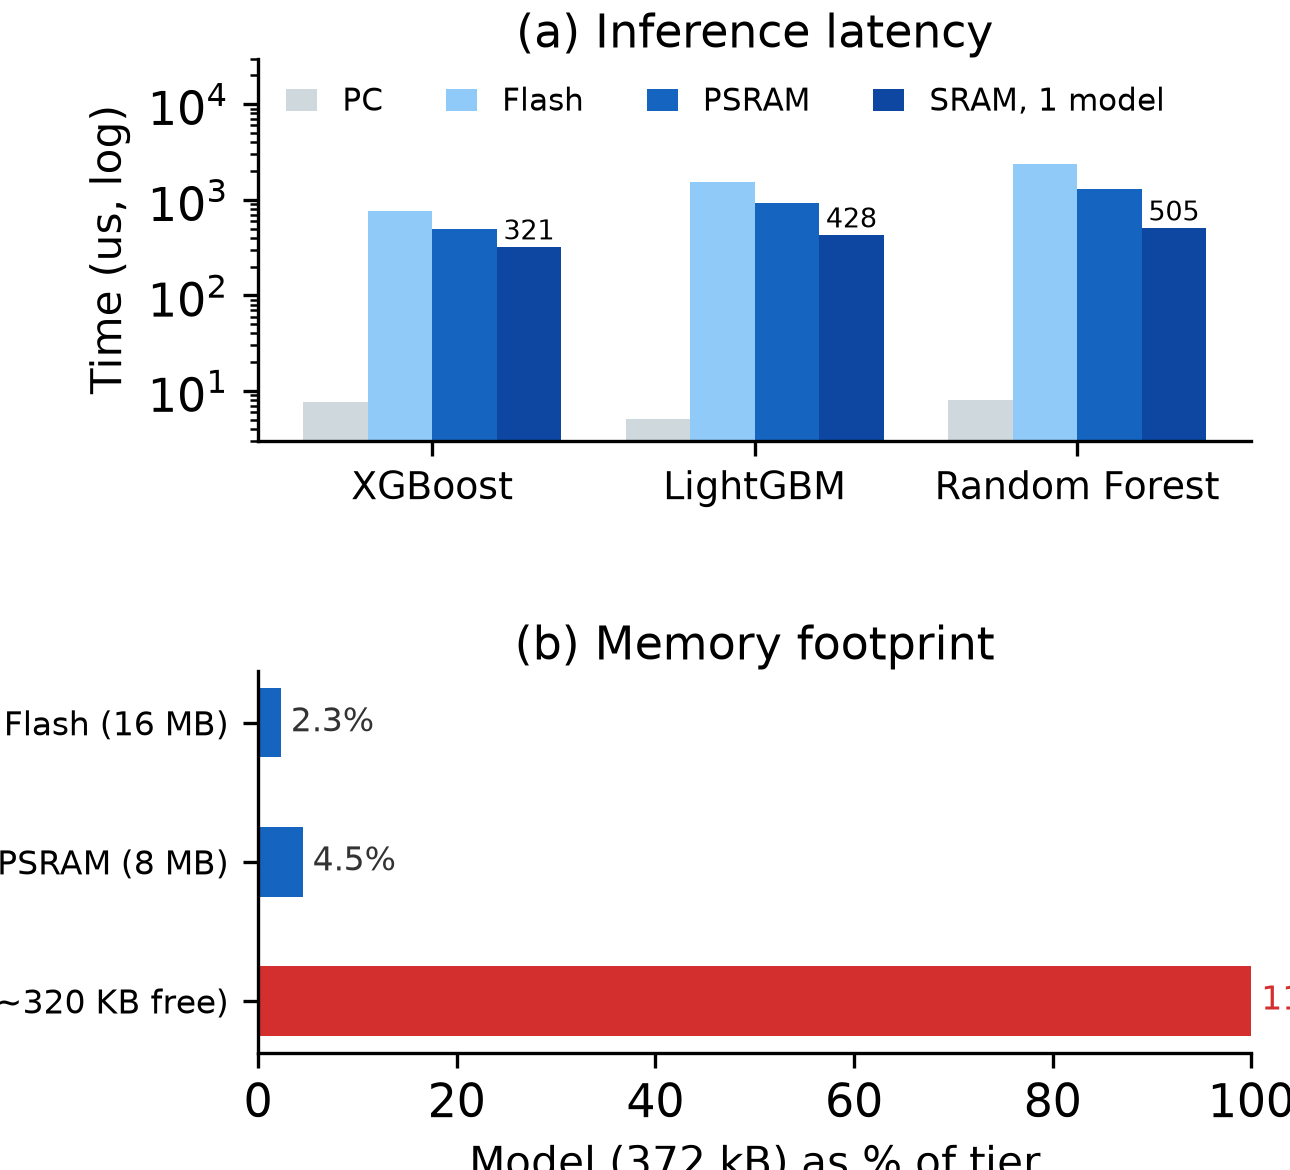
\includegraphics[width=0.9\textwidth]{fig_deploy.png}
\caption{Deployment trade-offs: (a) measured single-row inference time per model at 240 MHz with the binary in memory-mapped flash, PSRAM, or a single model in internal SRAM (dashed line: all three models from PSRAM); (b) per-model and combined binary footprint as a share of the ESP32-S3's roughly 320 kB of free internal SRAM --- each model fits, the combined 372 kB binary does not.}
\label{fig:deploy}
\end{figure*}

\begin{figure*}[!t]
\centering
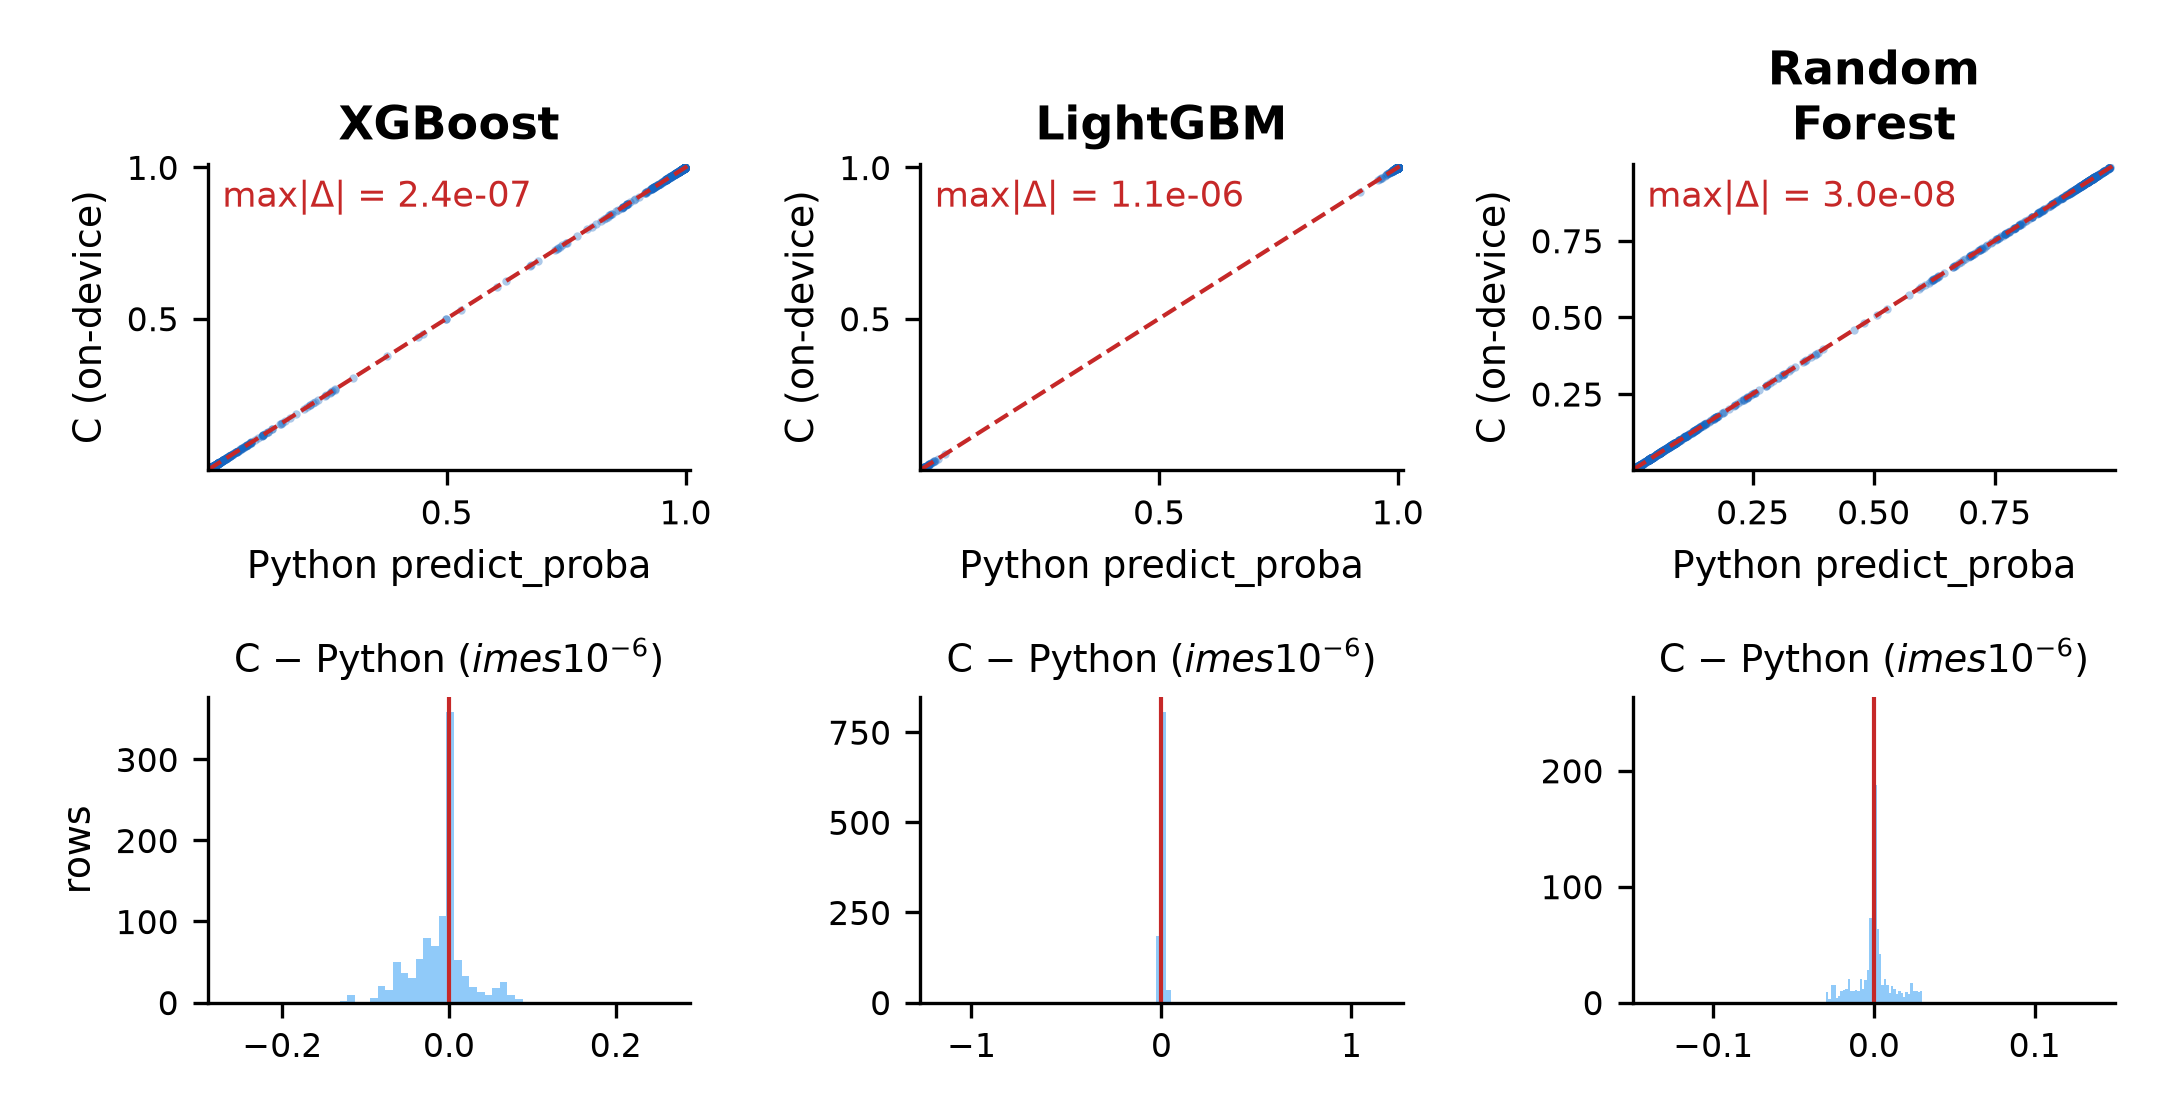
\includegraphics[width=0.9\textwidth]{fig_py_c_agreement.png}
\caption{On-device C engine predictions versus Python \texttt{predict\_proba()} over all 1 028 rows and three models (agreement scatter on the identity line, inset residual histogram of C minus Python in units of $10^{-6}$). Maximum absolute errors are $2.4\times10^{-7}$ (XGBoost), $1.1\times10^{-6}$ (LightGBM), and $3.0\times10^{-8}$ (Random Forest).}
\label{fig:pyc}
\end{figure*}

\section{Discussion, Analysis, and Novelty}

\subsection{The SOH Shortcut, Precisely Stated}
The evidence assembled above supports a precise statement --- more precise, and more useful, than the earlier version of this study offered. When a failure-risk model trained on one battery dataset is evaluated on another, its apparent transfer performance is dominated by the SOH coordinate; much of that dominance is definitional rather than learned, because SOH enters the failure label itself, and the failure-definition ablation of Section~III-F measures how much: relabeling failure by voltage sag alone removes most of the with-SOH transfer advantage on Severson. What remains is a weak, real health-state signal --- a cell far below nominal capacity is genuinely closer to failure under any reasonable definition. Everything else the sensors measure is dataset-specific: the same-chemistry controls show the collapse is caused by dataset shift at least as much as by chemistry, and the factorial ablation shows no non-SOH feature group carries usable cross-dataset signal. ``SOH is a chemistry-specific lookup key,'' the earlier framing, claimed more than the design could identify; the defensible claim is that apparent cross-dataset, cross-chemistry transferability is largely a health-state shortcut whose size this paper measures with label-, feature-, and dataset-level controls.

\subsection{Implications for Battery Management Practitioners}
Four practical points follow:
\begin{itemize}
\item \textbf{1)} Within-chemistry, within-laboratory failure-risk models built from standard charge--discharge features are reliable --- fold-mean AUC of 0.87 and above with Platt calibration --- and run on a \$12 microcontroller in under a millisecond. Deploy them where the training distribution holds.
\item \textbf{2)} Do not transfer models across datasets on the strength of an AUC table. If SOH is available at the target, an unfitted threshold rule is the correct first baseline, and any ensemble that cannot beat it has learned nothing portable; if SOH is unavailable, expect chance-level or inverted performance.
\item \textbf{3)} Quote risks from a formulation whose horizons are coherent. Four independent classifiers can and do assign ``risk within 10 cycles'' above ``risk within 50 cycles''; the survival-product formulation of Section~II-G removes that incoherence at no measured accuracy cost.
\item \textbf{4)} Under shift, prefer raw or Platt-scaled scores over isotonic, expect calibration to require labeled target data (5--10 cells suffice for ECE, but they do not restore discrimination), and choose decision thresholds on source data with an explicit cost model --- then verify, because Section~III-K shows the operating point itself does not survive the shift without SOH.
\end{itemize}

\subsection{Limitations}
The honesty of this paper has limits of its own. Oxford contributes only five cells --- effectively four for per-cell statistics --- at a 100-cycle logging resolution that makes its labels horizon-invariant, so it functions as a pooled-detection target; every Oxford claim is re-verified on the 141-cell Severson set. CALCE contributes seven cells, so its leave-one-cell-out folds are few and its uncertainty is correspondingly wide. The GRU is small and evaluated at three seeds, not thirty; its instability under shift is itself a finding, but wider sequence models trained on far more cells might behave differently --- nothing in this paper convicts the architecture, only this instance of it. The hazard model uses measured features at scored cycles; a strictly causal deployment reading must remember that post-failure rows are trivially positive for all formulations. The cost analysis fixes a 20:1 ratio and selects thresholds on source data; other ratios shift the operating point but not the conclusion that no usable operating point exists without SOH. Finally, the study is one-directional (LCO$\to$LFP plus within-chemistry controls); a controlled same-laboratory cross-chemistry experiment, which no public dataset currently supports, would be needed to isolate chemistry as a causal variable.

\section{Conclusion}
This study set out to widen a multi-horizon failure-risk classification framework and found that the widening itself demanded a validity analysis. Within dataset, the framework is sound: fold-mean AUC of 0.90--0.96 across three tree ensembles under cell-disjoint evaluation with leakage-free calibration, a discrete-time hazard formulation that matches the fixed-horizon classifiers while keeping cumulative risks monotone in the horizon, and a 372~kB embedded deployment that reproduces the training libraries to within $1.1\times10^{-6}$ on a \$12 ESP32-S3.

Across datasets, the apparent transferability is mostly a State-of-Health shortcut. A distance-to-threshold rule on SOH alone reproduces the tuned ensembles' transfer performance to within the cell-level bootstrap intervals; removing SOH collapses every model class toward or below chance, with sensor features sometimes inverting; relabeling failure by voltage sag alone --- a criterion SOH does not define --- removes most of the with-SOH advantage; and same-chemistry cross-laboratory controls show the collapse is caused by dataset shift at least as much as by chemistry. The supported conclusion is deliberately narrower than ``SOH is chemistry-specific'': much of the observed cross-dataset discrimination is attributable to SOH, partly because SOH defines the failure criterion itself, rather than to degradation information in the remaining measured features.

Calibration behaves as the validity story predicts: fitted on leakage-free out-of-fold scores, Platt preserves discrimination best at comparable calibration error, isotonic's tied step function destroys precision--recall and fails outright under shift, labeled-target recalibration repairs calibration error but not discrimination, and no score type yields a usable cost-based operating point on the shifted target without SOH. Statistical evidence is carried by cell-level bootstrap intervals, with cycle-level significance tests demoted to a consistency check under an explicit pseudoreplication caveat.

Future work, in order of directness: an SOH-free failure definition (voltage- or impedance-based endpoints) as the primary target for cross-dataset models; same-laboratory, cross-chemistry aging campaigns that isolate chemistry; learned representations trained for dataset invariance rather than chemistry invariance; cell-level hierarchical calibration that propagates uncertainty from cells to risk statements; and multi-seed, multi-architecture sequence-model studies on the scale where sequence models can plausibly generalize.

\clearpage
\section*{Acknowledgment}
This work received no external funding. The authors declare no conflicts of interest. The source code, data, trained models, and analysis pipeline are publicly available at \texttt{https://github.com/\allowbreak{}touhidsiddiqueeraj-bit/\allowbreak{}Multi-Horizon-\allowbreak{}Hazard-Models-for-Battery-\allowbreak{}Failure-Prediction}.

\raggedbottom
\begin{thebibliography}{20}
\bibitem{shikdar2026learning} T. A. Shikdar and H. Laaksonen, ``Learning when not to use a battery: Multihorizon failure intelligence,'' \emph{Int. Trans. Electr. Energy Syst.}, vol. 36, Art. no. 6000810, 2026.
\bibitem{meng2019review} H. Meng and Y. Li, ``A review on prognostics and health management (PHM) methods of lithium-ion (Li-ion) batteries,'' \emph{Renew. Sustain. Energy Rev.}, vol. 116, Art. no. 109405, 2019.
\bibitem{breiman2001random} L. Breiman, ``Random forests,'' \emph{Mach. Learn.}, vol. 45, no. 1, pp. 5--32, 2001.
\bibitem{chen2016xgboost} T. Chen and C. Guestrin, ``XGBoost: A scalable tree boosting system,'' in \emph{Proc. ACM SIGKDD}, 2016, pp. 785--794.
\bibitem{ke2017lightgbm} G. Ke, Q. Meng, T. Finley, et al., ``LightGBM: A highly efficient gradient boosting decision tree,'' in \emph{Proc. NeurIPS}, vol. 30, 2017, pp. 3146--3154.
\bibitem{saha2007battery} B. Saha and K. Goebel, ``Battery data set,'' NASA Ames Prognostics Data Repository, 2007.
\bibitem{calce2023battery} CALCE Battery Research Group, ``Battery aging datasets,'' Univ. Maryland, 2023.
\bibitem{birkl2017oxford} C. R. Birkl and D. A. Howey, ``Oxford battery degradation dataset 1,'' Univ. Oxford, 2017.
\bibitem{severson2019data} K. A. Severson, P. M. Attia, N. Jin, et al., ``Data-driven prediction of battery cycle life before capacity degradation,'' \emph{Nature Energy}, vol. 4, pp. 383--391, 2019.
\bibitem{sahoo2022transfer} S. Sahoo, K. S. Hariharan, S. Agarwal, et al., ``Transfer learning based generalized framework for state of health estimation of Li-ion cells,'' \emph{Sci. Rep.}, vol. 12, Art. no. 13173, 2022.
\bibitem{lu2023deep} J. Lu, R. Xiong, J. Tian, C. Wang, and F. Sun, ``Deep learning to estimate lithium-ion battery state of health without additional degradation experiments,'' \emph{Nat. Commun.}, vol. 14, Art. no. 2760, 2023.
\bibitem{platt1999probabilistic} J. C. Platt, ``Probabilistic outputs for support vector machines and comparisons to regularized likelihood methods,'' in \emph{Adv. Large Margin Classifiers}, MIT Press, 1999, pp. 61--74.
\bibitem{zadrozny2002transforming} B. Zadrozny and C. Elkan, ``Transforming classifier scores into accurate multiclass probability estimates,'' in \emph{Proc. ACM SIGKDD}, 2002, pp. 694--699.
\bibitem{niculescu2005predicting} A. Niculescu-Mizil and R. Caruana, ``Predicting good probabilities with supervised learning,'' in \emph{Proc. ICML}, 2005, pp. 625--632.
\bibitem{huang2020experimental} L. Huang, J. Zhao, B. Zhu, H. Chen, and S. K. L. M. v. Broucke, ``An experimental investigation of calibration techniques for imbalanced data,'' \emph{IEEE Access}, vol. 8, pp. 127343--127352, 2020.
\bibitem{lundberg2020from} S. M. Lundberg, G. G. Erion, H. Chen, et al., ``From local explanations to global understanding with explainable AI for trees,'' \emph{Nat. Mach. Intell.}, vol. 2, no. 1, pp. 56--67, 2020.
\bibitem{grzesik2024combining} P. Grzesik and D. Mrozek, ``Combining machine learning and edge computing: Opportunities, challenges, platforms, frameworks, and use cases,'' \emph{Electronics}, vol. 13, no. 3, Art. no. 640, 2024.
\bibitem{gupta2023online} C. Gupta and A. Ramdas, ``Online Platt scaling with calibeating,'' in \emph{Proc. ICML}, PMLR 202, 2023, pp. 12182--12204.
\bibitem{delong1988comparing} E. R. DeLong, D. M. DeLong, and D. L. Clarke-Pearson, ``Comparing the areas under two or more correlated receiver operating characteristic curves: A nonparametric approach,'' \emph{Biometrics}, vol. 44, no. 3, pp. 837--845, 1988.
\bibitem{shikdar2026robustness} T. A. Shikdar and H. Laaksonen, ``How far does the model hold? Robustness of multihorizon battery failure intelligence under realistic operating conditions,'' submitted for publication, 2026.
\end{thebibliography}

\EOD

\end{document}
